\chapter{Systèmes d'équations linéaires}
Considérez l'équation suivante:
\[
x = 2
\]
Ceci est une équation linéaire avec une seule inconnue.

\begin{NotDef}
Une \textbf{inconnue} est un \textit{scalaire} déguisé sous
la forme d'une lettre\sidenote{Pour augmenter la confusion, on utilise parfois des lettres
grecques au lieu de lettre de l'alphabet latin utilisé en
français.}.

Un \textbf{scalaire} est le mot utilisé en mathématiques
supérieures pour désigner un nombre\sidenote{Dans ce livre, on suppose toujours que c'est un nombre réel.}.
\end{NotDef}

Rajoutons une deuxième équation linéaire, avec une autre
inconnue.
\[
\left\{
\begin{matrix}
    x &=& 2\\
    y &=& 1
\end{matrix}
\right.
\]
\begin{marginfigure}
\begin{mdframed}
    \scalebox{0.8}{
		\begin{tikzpicture}
			% les axes
			\draw[->] (-1,0) -- (4,0) node[anchor=west]{\color{gray}x};
			\draw[->] (0,-1) -- (0,4) node[anchor=south]{\color{gray}y};
			% les deux droites
			\draw[-, thick, blue] (-1,1) -- (4,1) node[anchor=north]{\color{blue}\small $y=1$};
			\draw[-, thick, purple] (2,-1) --(2,4) node[anchor= east]{\color{purple}\small $x=2$};
			% le point d'intersection
			\coordinate (A) at (2,1);
			\draw[-] (2, -0.1) node[anchor=north]{\small 2} -- (2, 0.1);
			\draw[-] (-0.1, 1) node[anchor=east]{\small 1} -- (0.1, 1);
			\node [fill=black,inner sep=2pt,label=30:$\mbox{\quad(2,1)}$] at (2,1) {};
		\end{tikzpicture}
}
\caption{Deux droites qui s'intersectent dans un plan.}
\end{mdframed}
\end{marginfigure}

Ceci est un exemple d'un \textbf{système} d'équations linéaires.

\begin{NotDef}
Un \textbf{système d'équations linéaires} est une collection
d'équations linéaires ayant des inconnues communes.%
\sidenote{Pour que l'utilisation du mot \textit{communes} soit correct, il faudrait
plutôt écrire:
\[
\left\{
\begin{matrix}
    x + 0y &=& 2\\
    y + 0x &=& 1
\end{matrix}
\right.
\]
}
\end{NotDef}

Puisqu'on a un système avec deux inconnues, $x$ et $y$, on
peut le représenter par deux droites dans un plan.
La \textbf{solution} de ce système correspond au point
d'intersection de ces deux droites.

Algébriquement, on peut représenter cette solution de deux
façons:
\begin{itemize}
\item[$\bullet$] En utilisant la notation traditionnelle
pour un point: $(x, y) = (2, 1)$.
\item[$\bullet$] En écrivant la solution comme un système
d'équations linéaires où chaque inconnue n'apparait qu'une
seule fois, avec une ligne différente pour chaque inconnue. 
Ceci est identique à ce que nous avions écrit précédemment:
\[
\left\{
\begin{matrix}
    x &=& 2\\
    y &=& 1
\end{matrix}
\right.
\]
\end{itemize}

\section{Opérations élémentaires sur les lignes}

Le système d'équations linéaires que nous avons écrit
ci-dessus comporte deux équations, chacune écrite sur
une ligne différente. Nous pouvons numéroter ces équations
dans l'ordre où elles apparaissent.
\[
\left\{
\begin{matrix}
    x &=& 2\qquad {\scriptstyle\color{red}\fbox{1}}\\
    y &=& 1 \qquad {\scriptstyle\color{red}\fbox{2}}
\end{matrix}
\right.
\]
Nous pouvons interchanger les deux lignes sans que 
la solution ne change
\[
\left\{
\begin{matrix}
    y &=& 1\qquad {\scriptstyle\color{red}\fbox{1}}\\
    x &=& 2 \qquad {\scriptstyle\color{red}\fbox{2}}
\end{matrix}
\right.
\]
On dit que ces deux systèmes d'équations linéaires\sidenote{L'original et celui avec les équations dans un autre ordre différent.}
sont \textbf{équivalents}.
\begin{TrueDef}{Équivalence}
Deux systèmes d'équations linéaires sont dits \textbf{équivalents} s'ils ont la même solution.
\end{TrueDef}
L'interchange de deux lignes est un exemple
d'une \textbf{opération élémentaire sur les lignes}.
Dans ce qui suit, on dénotera un tel interchange
de la façon suivante:
\[
L_1 \leftrightarrow L_2
\]

\begin{NotDef}
Une \textbf{opération élémentaire sur les lignes}\footnote{Une opération élémentaire sur les lignes n'est pas un concept mathématique mais un truc de calcul; il n'y a
donc pas de définition formelle pour ceci.} est
une opération mathématique qui transforme un système
d'équations linéaires en un système équivalent.
\end{NotDef}

Une autre opération sur les lignes qu'on peut effectuer est
de remplacer une ligne donnée par l'addition de celle-ci avec le multiple 	d'une autre ligne.


\begin{align*}
&\left\{
\begin{matrix}[ccc]
    y&=& 1\qquad {\scriptstyle\color{red}\fbox{1}}\\
    x &=& 2\qquad {\scriptstyle\color{red}\fbox{2}}
\end{matrix}
\right.
\\
&\qquad\mbox{\color{blue} est équivalent à}\\
&\left\{
\begin{matrix}[rrrrll]
    &&y&=& 1	\\	
    x&-&y &=& 1 & {\color{blue}\Leftarrow\quad L_2 - L_1} 
\end{matrix}
\right.
\end{align*}
		

Finalement, une troisième opération élémentaire qu'on peut effectuer
est de multiplier une ligne par une constante différente
de zéro.

\begin{align*}
&\left\{
\begin{matrix}[rrrrl]
    &&y&=& 1	\qquad {\scriptstyle\color{red}\fbox{1}}\\	
    x&-&y &=& 1\qquad {\scriptstyle\color{red}\fbox{2}}
\end{matrix}
\right.
\\
&\qquad\mbox{\color{blue} est équivalent à}\\
&\left\{
\begin{matrix}[rrrrll]
    &&3y&=& 3	&{\color{blue}\Leftarrow\quad 3 L_1}\\	
    x&-&y &=& 1
\end{matrix}
\right.
\end{align*}

Pour vraiment compliquer les choses davantages,
faisons une dernière opération sur les lignes
\begin{marginfigure}
		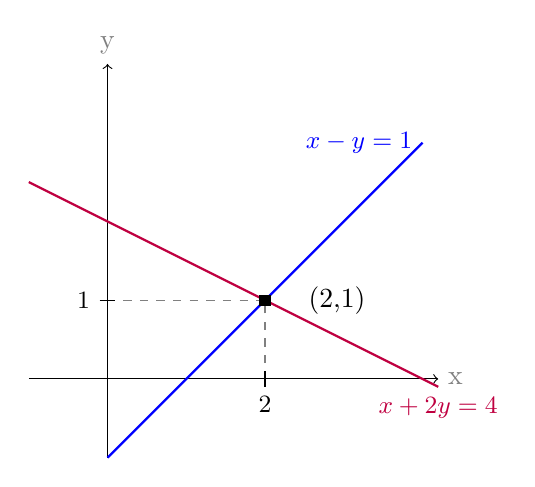
\begin{tikzpicture}
			% les axes
			\draw[->] (-1,0) -- (4.2,0) node[anchor=west]{\color{gray}x};
			\draw[->] (0,-1) -- (0,4) node[anchor=south]{\color{gray}y};
			% les deux droites
			\draw[-, thick, blue] (0,-1) -- (4,3) node[anchor=east]{\color{blue}\small $x-y=1$};
			\draw[-, thick, purple] (-1,2.5) --(4.2,-0.1) node[anchor=north]{\color{purple}\small $x+2y=4$};
			% le point d'intersection
			\coordinate (A) at (2,1);
			\draw[-] (2, -0.1) node[anchor=north]{\small 2} -- (2, 0.1);
			\draw[-] (-0.1, 1) node[anchor=east]{\small 1} -- (0.1, 1);
			\draw [dashed, gray] (2, 0.2) -- (A);
			\draw [dashed, gray] (0.2, 1) -- (A);
			\node [fill=black,inner sep=2pt,label=0:$\mbox{\quad(2,1)}$] at (2, 1) {};
		\end{tikzpicture}
			\caption{Interprétation graphique de ce nouveau système d'équations linéaires}
\end{marginfigure}

\begin{align*}
&\left\{
\begin{matrix}[rrrrl]
    &&3y&=& 3	\qquad {\scriptstyle\color{red}\fbox{1}}\\	
    x&-&y &=& 1\qquad {\scriptstyle\color{red}\fbox{2}}
\end{matrix}
\right.
\\
&\qquad\mbox{\color{blue} est équivalent à}\\
&\left\{
\begin{matrix}[rrrrll]
    x&+&2y&=& 4	&{\color{blue}\Leftarrow\quad L_1 + L_2}\\	
    x&-&y &=& 1
\end{matrix}
\right.
\end{align*}
Bien que les deux équations soient très différentes de celles
du départ, et que le graphique correspondant soit également
différent, la solution reste inchangée.

Nous avons donc maintenant un système d'équations linéaires avec deux inconnues, où les deux inconnues apparaissent dans chacune des deux équations. Ce système est équivalent à celui du départ, plus simple et où on peut immédiatement identifier
la valeur de chacune des inconnues.

\[
\left.
\begin{matrix}
    x &=& 2\\
    y &=& 1
\end{matrix}
\right\} \qquad\mbox{équivalent à}\qquad 
\left\{
\begin{matrix}
    x&+&2y&=& 4	\\	
    x&-&y &=& 1
\end{matrix}
\right.
\]
\section{Matrice augmentée}

\begin{NotDef}
Une \textbf{inconnue} est un scalaire qui s'est déguisée sous
la forme d'une lettre, \textit{parfois augmentée d'un \textbf{indice}, et
dont on demande aux étudiants d'en deviner l'identité.}

Un \textbf{indice} est un chiffre qu'on met au bas d'une lettre, comme
ceci: $x_{\color{red} 1}$,
pour la distinguer d'une autre lettre, $x_{\color{red} 2}$, identique mais indiquant une quantité différente; on utilise
parfois un indice lorsqu'on pense qu'on n'a pas
suffisamment de lettres dans l'alphabet pour
désigner toutes les inconnues.\sidenote{Il ne faut pas
confondre un indice, et un \textbf{exposant}, ce dernier apparaissant
en haut de la lettre, $x^1$.}
\end{NotDef}

Supposons que l'on vous demande de trouver la
solution du système d'équations linéaires suivant:
\[
\left\{
\begin{matrix}
    x_1&+&2x_2&=& 4	\\	
    x_1&-&x_2 &=& 1
\end{matrix}
\right.
\]
ayant les inconnues $x_1$ et $x_2$.  Sauf pour le choix
des inconnues, on reconnait ce système d'équations linéaires
comme étant identique au précédent. On connait donc déjà la
solution:
\[
\left\{
\begin{matrix}
x_1 &=& 2\\
x_2 &=& 1
\end{matrix}
\right.
\]
Si on ne connaissait pas cette solution, on aurait pu la
retrouver en faisant l'inverse des opérations élémentaires
sur les lignes qu'on avait vu\sidenote{On fera ceci dans
un exemple ci-dessous.}.
Parce que ces opérations élémentaires ne dépendent pas des
choix des symboles utilisés pour dénoter les inconnues,
on trouve utile d'introduire une notation qui n'inclut pas
ces symboles. Ainsi, au lieu d'écrire:
\[
\left\{
\begin{matrix}
    x_1&+& 2x_2&=& 4	\\	
    x_1&-&x_2 &=& 1
\end{matrix}
\right.
\color{black}
\]
on écrit la version totalement équivalente suivante:
\[
\left\{
\begin{matrix}
    {\color{red}1}x_1&+& {\color{red}2}x_2&=& {\color{blue}4}	\\	
    {\color{red}1}x_1&+&({\color{red}-1})x_2 &=& {\color{blue}1}
\end{matrix}
\right.
\color{black}
\]
Les chiffres, en rouge, devant les inconnues sont appelés
les \textbf{coefficients}; ceux en bleu sont les termes constants.
Ayant identifié les coefficients et les termes constants,
on se débarrasse de tout le reste, considéré comme une notation
superflue, et on écrit plutôt:
\[
\begin{bmatrix}[rr|r]
{\color{red}1} & {\color{red}2} & {\color{blue}4}\\
{\color{red}1} & {\color{red}-1} & {\color{blue}1}
\end{bmatrix}
\]
On appelle ceci la \textbf{matrice\sidenote{On verra la définition d'une matrice dans le prochain chapitre} augmentée} du système
d'équations linéaires. La partie à gauche de la barre verticale\sidenote{Certains mathématiciens, préférant le minimalisme absolu, n'incluent pas
une telle barre verticale dans une matrice augmentée.}, 
avec les chiffres en rouge, s'appelle \textbf{matrice des coefficients}. 

\begin{NotDef}
La notation des matrices augmentées a été inventée par des mathématiciens qui cherchaient à trouver des solutions
pour des systèmes d'équations linéaires mais qui n'aimaient
pas utiliser des lettres (pour les inconnues), ni des signes
d'addition ($+$) ou d'égalité ($=$).
\end{NotDef}

On peut également écrire la solution sous la forme
d'une matrice augmentée en procédant comme ceci:
\[
\left\{
\begin{matrix}
x_1 &=& 2\\
x_2 &=& 1
\end{matrix}
\right.
\quad {\color{purple}\Rightarrow}\quad
\left\{
\begin{matrix}
{\color{red}1} x_1 &+& {\color{red}0}x_2 &=& {\color{blue}2}\\
{\color{red}0} x_1 &+& {\color{red}1}x_2 &=& {\color{blue}1}
\end{matrix}
\right.
\quad {\color{purple}\Rightarrow}\quad
\begin{bmatrix}[rr|r]
{\color{red}1} & {\color{red}0} & {\color{blue}2}\\
{\color{red}0} & {\color{red}1} & {\color{blue}1}
\end{bmatrix}
\]

La matrice augmentée de la solution est dans ce qu'on
appelle une \textit{forme échelonnée réduite} que l'on définira un peu plus tard.

Dans un cours d'introduction à l'algèbre linéaire, \textbf{la très grande majorité des calculs\sidenote{Ce qui semble ëtre difficile pour les étudiants est d'interpréter correctement ces calculs qui sont,
en général, très simples.} que vous aurez
à faire} consiste à faire des opérations élémentaires sur les lignes
pour obtenir, si cela est possible, une matrice
\textbf{équivalente} dans la \textbf{forme échelonnée réduite.}

\begin{Example}
\[
\begin{matrix}
\color{blue}\left\{
\begin{matrix}[rrrrr]
x_1 &+& 2x_2 &=& 4\\
x_1 & -& x_2 &=& 1
\end{matrix} \right. &\color{blue}\Rightarrow&
\begin{bmatrix}[rr|r]
1 & 2 & \hphantom{-}4\\
1 & -1 & 1
\end{bmatrix} \\[20pt]
\color{red}L_2 - L_1 \rightarrow L_2 &\color{red}\Rightarrow&
\begin{bmatrix}[rr|r]
1 & 2 & 4\\
0 & -3 & -3
\end{bmatrix} \\[20pt]
\color{red}-\frac13 L_2 \rightarrow L_2 &\color{red}\Rightarrow&
\begin{bmatrix}[rr|r]
1 & \hphantom{-}2 & \hphantom{-}4\\
0 & 1 & 1
\end{bmatrix} \\[20pt]
\color{red}L_1 - 2L_2 \rightarrow L_1 &\color{red}\Rightarrow&
\begin{bmatrix}[rr|r]
1 & \hphantom{-}0 & \hphantom{-}2\\
0 & 1 & 1
\end{bmatrix} &\color{blue}\Rightarrow&
\color{blue}\left\{
\begin{matrix}
x_1 &=& 2\\
x_2 &=& 1
\end{matrix}
\right.
\end{matrix}
\]
\end{Example}

Nous terminons ce chapitre avec deux véritables définitions mathématiques.

\begin{TrueDef}{Équation linéaire}
Une \textbf{équation linéaire} est une équation qu'on peut mettre sous la forme
\[
a_1 x_1 + \ldots + a_n x_n = b
\]
où $b$ ainsi que les coefficients $a_1, \ldots a_n$ sont
des scalaires connus, et $x_1, \ldots, x_n$ sont des
inconnues.
\end{TrueDef}

\begin{TrueDef}{Système d'équations linéaires}
Un système de d'équations linéaires est une
collection de $m$ équations linéaires qui portent
sur les mêmes $n$ inconnues:
\[
\left\{
	\begin{matrix}
	a_{11}x_1 &+& a_{12}x_2 &+& \ldots &+& a_{1n}x_n &=& b_1 \\
	a_{21}x_1 &+& a_{22}x_2 &+& \ldots &+& a_{2n}x_n &=& b_2 \\
	\vdots && \vdots &&  && \vdots && \vdots \\
	a_{m1}x_1 &+& a_{m2}x_2 &+& \ldots &+& a_{mn}x_n &=& b_m
	\end{matrix}
	\right.
\]
\end{TrueDef}

